% arXiv version. Shares every section, table and figure with main.tex (ACL/ARR version);
% only the preamble, title block and bibliography style differ.
% Build: pdflatex main_arxiv && bibtex main_arxiv && pdflatex main_arxiv && pdflatex main_arxiv
% Upload package: bash make_arxiv.sh
\PassOptionsToPackage{dvipsnames}{xcolor}
\documentclass[11pt,letterpaper]{style}

\usepackage[numbers]{natbib}
\usepackage{graphicx}
\usepackage{booktabs}
\usepackage{multirow}
\usepackage{amsmath}
\usepackage{amssymb}
\usepackage{colortbl}
\usepackage{xcolor}
\usepackage{algorithm}
\usepackage{algpseudocode}
\usepackage{listings}
\usepackage{pgfplots}
\pgfplotsset{compat=1.17}
\usepgfplotslibrary{groupplots}
\usepackage{cleveref}
\definecolor{otblue}{HTML}{2456A6}
\definecolor{otpurple}{HTML}{8A5AA8}
\definecolor{otorange}{HTML}{C2571A}
\definecolor{otgreen}{HTML}{3D8F6B}
\definecolor{otred}{HTML}{B3261E}
\definecolor{otgray}{HTML}{63666B}
% marks in the result tables: the row is reliably lower / higher than OmniTrace (paired 95% bootstrap interval)
\newcommand{\mdn}{{\tiny$\downarrow$}}
\newcommand{\mup}{{\tiny$\uparrow$}}

\lstset{
    language=Python,
    basicstyle=\ttfamily\scriptsize,
    keywordstyle=\color{blue},
    commentstyle=\color{gray},
    stringstyle=\color{orange},
    showstringspaces=false,
    breaklines=true,
    frame=single
}
% layout macros used by the shared sections (main.tex sets the ACL values)
\newcommand{\tablesize}{\small}
\newcommand{\skiptablebegin}{\vspace{0pt}}
\newcommand{\skiptableend}{\vspace{0pt}}
\newcommand{\skipimgbegin}{\vspace{0pt}}
\newcommand{\skipimgend}{\vspace{0pt}}
\newcommand{\colfigwidth}{0.6\textwidth}  % single-column figures (one ACL column)
% one-column page: let the full-width figures sit at the top of a text page
\renewcommand{\topfraction}{0.9}
\renewcommand{\bottomfraction}{0.8}
\renewcommand{\textfraction}{0.07}
\renewcommand{\floatpagefraction}{0.8}
\setcounter{topnumber}{3}
\setcounter{totalnumber}{4}

% title block
\newcommand{\afficon}[1]{\textsuperscript{\fontsize{9pt}{9pt}\selectfont #1}}
\newcommand{\equal}{\textsuperscript{*}}     % Equal contribution
\newcommand{\advisor}{\textsuperscript{\dag}}% Equal advising
\renewcommand\Authfont{\centering\normalfont\bfseries\fontsize{11}{15}\selectfont}
\renewcommand\Affilfont{\centering\normalfont\fontsize{10}{15}\selectfont}
\newcommand{\afflogo}[2]{%
  \raisebox{#2}{\includegraphics[height=1.5em]{#1}}%
}

\title{\centering OmniTrace: \\ A Unified Framework for Generation-Time Source Attribution in Omni-Modal LLMs}
\runningtitle{OmniTrace: A Unified Framework for Generation-Time Source Attribution in Omni-Modal LLMs}

\author{%
    {\Authfont
    \textbf{Qianqi Yan}\textsuperscript{1} \quad
    \textbf{Yichen Guo}\textsuperscript{1} \quad
    \textbf{Ching-Chen Kuo}\textsuperscript{2} \quad
    \textbf{Shan Jiang}\textsuperscript{2} \quad
    \textbf{Hang Yin}\textsuperscript{2}

    \textbf{Yang Zhao}\textsuperscript{2} \quad
    \textbf{Xin Eric Wang}\textsuperscript{1}
    }\\
    {\Affilfont
    \textsuperscript{1} \afflogo{logo/ucsb.png}{-0.7ex} University of California, Santa Barbara \quad
    \textsuperscript{2} \afflogo{logo/ebay.png}{-0.7ex} eBay \quad
    }
}

\begin{document}

% style.cls stores the abstract and prints it inside \maketitle, so it is read first
\begin{abstract}
Omni-modal large language models answer questions over documents, audio, and video, but they do not show which part of the input an answer relies on.
Attribution methods for generated text either rerun the model many times with parts of the input removed or learn an attribution model, and they are defined and tested on text. Asking the model to cite its own evidence is cheap, but the citations are often missing and need not reflect what the model used.
We present OmniTrace, a training-free method that attributes every generated sentence to source units (text passages, images, and seconds of audio or video) in the same forward pass that generates it.
OmniTrace sums late-layer attention over the input positions of each unit and labels the units that stand out from the other units of the same modality. One rule and one threshold serve all modalities and models.
We test it with a causal protocol designed for continuous inputs: we hide the attributed units behind content-free placeholders, replay the model's own response, and compare the loss in log-probability with the loss from hiding the same number of random units.
On Qwen2.5-Omni and MiniCPM-o~4.5, over video, audio, and image--text question answering, the units OmniTrace selects matter more than random units in every setting, for whole responses and for single sentences.
OmniTrace has about twice the effect of embedding similarity and reaches 77--98\% of the effect of leave-one-out and ContextCite, which need 16 to 41 extra forward passes per question.
The model's own citations are absent from 18--69\% of responses, and on audio and image--text inputs the cited units matter 1.7 to 3.1 times less than the units OmniTrace selects on the same responses.
\end{abstract}

\makeatletter
\g@addto@macro\theabstract{%
  \par\vskip1em\noindent{\keywordsfont Keywords: Multimodal Large Language Models, Source Attribution, Generation-Time Explanation, Model Interpretability}%
  \par\vspace{3mm}\noindent\textbf{Project Page:} \url{https://github.com/eric-ai-lab/OmniTrace}%
}
\makeatother

\maketitle

\begin{figure*}[!ht]
\setlength{\abovecaptionskip}{0.3cm}
    \centering
    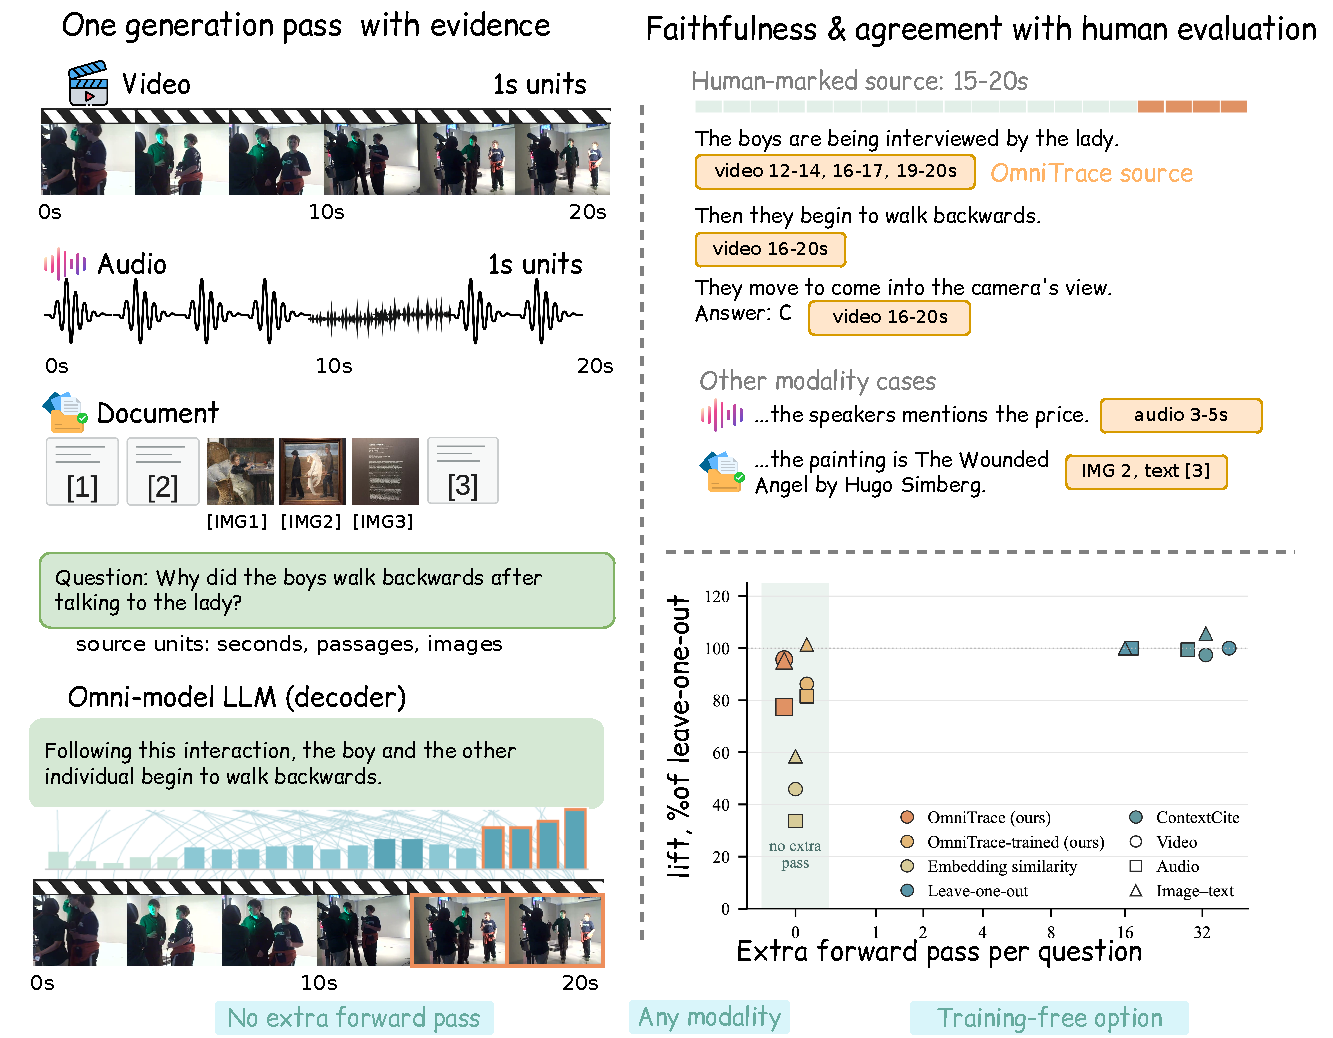
\includegraphics[width=\textwidth]{media/figure/Teaser.pdf}
    \caption{\textbf{OmniTrace reads what a model used from the pass that generates the answer.}
    \emph{Left:} video, audio, and documents enter one input sequence as source units (seconds, passages, images). While the decoder writes a sentence, OmniTrace sums the attention mass on each unit (bars) and labels the units that stand out within their modality (orange).
    \emph{Top right:} every sentence comes with its sources, as time intervals or source ids; here most labelled seconds fall inside the span that annotators marked, although no annotation was used.
    \emph{Bottom right:} tested by hiding units and replaying the response, OmniTrace reaches 77--96\% of the effect of leave-one-out with no extra forward pass, where perturbation needs 16 to 41 per question (Qwen2.5-Omni-7B).
    }
    \label{fig:teaser}
\end{figure*}

\section{Introduction}
\label{sec:intro}

Omni-modal large language models take text, images, audio, and video in one prompt and answer in free text~\cite{gpt-5.2, gemini3, Xu2025Qwen3OmniTR, yu2025minicpm, xu2025qwen2, ye2026omnivinci}.
When such a model answers a question about a forty-second clip or a fifteen-quote document pool, a user who wants to check the answer has to go through the whole input again. A useful system would point to the evidence: these three seconds of audio, this chart, this passage.
We study this problem as \emph{source attribution}: for each generated sentence, find the parts of the input that the model relied on when it produced that sentence.

Three kinds of methods exist, and none of them covers this setting.
\emph{Perturbation methods} such as leave-one-out and ContextCite~\cite{cohen-wang2024contextcite} hide parts of the context and measure how the output changes. They are faithful by construction but need tens of extra forward passes per query, and a video or a long audio clip makes each pass expensive.
\emph{Learned methods} such as AT2~\cite{cohenwang2025at2} and vStream~\cite{kang2026vstream} fit an attribution model on perturbation data, which has to be collected again for every model.
Both families were built for text contexts or for single images, and they have not been tested on continuous audio and video.
\emph{Self-citation} asks the model to state its own evidence. Recent work shows that stated audio and video citations are often hallucinated~\cite{wan2026murgat}, and a citation says what the model claims, not what it used.

Reading attention during generation is the natural cheap alternative: it needs no extra pass and no training. Attention has been used this way for text contexts~\cite{ding2025attention, wang2026attntrace}, and a natural design for mixed inputs traces every generated token to the single input position with the highest attention and then votes over tokens.
We find that this design does not hold up once the input is not text. With hard per-token assignment, the ranking of video seconds agrees with human evidence no better than chance, the question text wins almost every assignment when it competes with video tokens, and a rule tuned on one model loses most of its effect on another (\Cref{sec:design}).
There is also an evaluation gap. Attribution on audio and video has been scored by agreement with reference labels, which shows what a person would point to, not what the model depended on. A causal test needs a way to hide a time interval without leaving a trace of it, and a control for how much was hidden.

We introduce \textbf{OmniTrace}, a training-free attribution method that runs inside the generation pass, together with a causal protocol to test it on every modality.
OmniTrace splits the input into \emph{source units} by structure the input already has: one-second units for audio and video, and one unit per text passage or image.
For each generated token it sums the attention of the late decoder layers over the positions of each unit. Summing these \emph{attention masses} over the tokens of a sentence gives one score per unit, and a unit is labelled as evidence when its score stands out from the other units of its modality.
There is no per-token argmax, no token weighting, no learned component, and no per-modality tuning: the layer band is a fixed fraction of the model's depth and one threshold is used throughout.
The same pass that generates the response returns its attribution, as source ids for text and images and as time intervals for audio and video.

To test whether these units are the ones the model used, we replay the model's own response with units hidden and measure the loss in log-probability.
Hidden units are replaced at the input by placeholders of the same length that carry no content (black frames, silence, a black image, blank tokens), and every result is compared with hiding the same number of random units.
Leave-one-out and ContextCite are run on the same units with the same placeholders, so no baseline is ``not applicable'' on audio or video.

On Qwen2.5-Omni~\cite{xu2025qwen2} and MiniCPM-o~4.5~\cite{yu2025minicpm}, with video (NExT-GQA), audio (MMAU), and image--text documents (MMDocRAG), we find:
\begin{itemize}
    \item \textbf{One pass is enough for most of the faithfulness.} The units OmniTrace selects matter more than random units in all settings, for whole responses and for single sentences. OmniTrace has about twice the effect of embedding similarity and 77--98\% of the effect of leave-one-out and ContextCite, at none of their 16 to 41 extra forward passes.
    \item \textbf{What the model cites is not what it uses.} When asked to cite, the model cites nothing in 18--69\% of responses. On audio and image--text inputs, the cited units matter 1.7 to 3.1 times less than the units OmniTrace selects on the same responses.
    \item \textbf{The simple rule transfers; hard tracing does not.} The same setting works on a second model family without retuning, while per-token argmax tracing loses almost all of its effect on audio there.
    \item \textbf{Attention has measurable limits.} Summed attention favors large units, effects on video are small, and on one model human-marked evidence matters more than the units OmniTrace picks. We quantify each of these.
\end{itemize}

In short, we contribute a single-pass, training-free attribution method for text, image, audio, and video sources, a causal evaluation protocol for continuous inputs, and an analysis of stated versus used evidence, unit-size bias, and modality reliance.

\section{Related Work}

\paragraph{Context attribution for text LLMs.}
A recent line of work attributes a generated statement to the context passages that support it.
ContextCite~\cite{cohen-wang2024contextcite} hides random subsets of the context and fits a sparse linear model of the response probability; ARC-JSD~\cite{li2026arcjsd} and AttriBoT~\cite{liu2025attribot} make such perturbation estimates more accurate or cheaper.
MIRAGE~\cite{qi-etal-2024-model} uses gradient saliency to link answer tokens to retrieved documents.
Closer to our signal, AT2~\cite{cohenwang2025at2} learns one weight per attention head from perturbation data, and AttnTrace~\cite{wang2026attntrace} and \citet{ding2025attention} read attention directly for text contexts.
All of these define sources as discrete text units and are evaluated on text.
OmniTrace uses the same kind of signal as the attention-based methods, needs no training, and is defined over units of any modality, including time intervals.
The term \emph{generation-time} is also used for prompted citation~\cite{saxena2025generation, gao2023alce}; we use it for attribution that is read from the model's internals while it decodes.

\paragraph{Attribution for vision--language models.}
vStream~\cite{kang2026vstream} streams attribution to image regions during reasoning but learns a map from attention to perturbation effects. VTrace~\cite{yuan2026vtrace} and ERCR~\cite{liang2025ercr} are post-hoc methods for image patches, and MultAttnAttrib~\cite{tran2026multattnattrib} applies selected attention heads to long documents.
These methods cover images and text. None covers audio or video timelines, and none tests attribution causally on continuous inputs.

\paragraph{Temporal evidence in audio and video.}
Models can be trained or prompted to state the time intervals that support an answer~\cite{lu2025vited, wang2025groundedvideollm, zhu2026timelens2}.
MuRGAt~\cite{wan2026murgat} shows that such stated citations are often hallucinated even when the reasoning is correct, and NExT-GQA~\cite{xiao2024nextgqa} shows that video models often answer correctly without looking at the relevant moment.
Mechanistic studies trace where audio information enters the answer across layers~\cite{cho2026tracingaudio, chen2026causalaudio}, but they do not attribute individual generated claims.
We measure which intervals a model relied on for each sentence and compare them with the intervals it states.

\paragraph{Evaluating attribution.}
Attribution can be scored by agreement with human evidence or by its causal effect on the output~\cite{deyoung2020eraser, atanasova-etal-2020-diagnostic}. The two can disagree: \citet{alhamidi2026carve} find that the sensitivity of video models to removed frames tracks annotated evidence only weakly.
We therefore use causal tests as the main evaluation and report agreement with human evidence separately.

\section{OmniTrace}
\label{sec:method}

\subsection{Problem Setting}
\label{sec:problem}

\paragraph{Input and source units.}
A decoder-only omni-modal LLM receives an input sequence $\mathbf{x}=(x_1,\dots,x_N)$ in which text tokens and the encoder outputs for images, audio, and video share one sequence.
We split the attributable part of $\mathbf{x}$ into \emph{source units} $\mathcal{S}=\{S_1,\dots,S_m\}$, each a set of input positions, using structure the input already has.
A text passage is one unit and an image is one unit.
Audio and video are cut into units of about one second, following the time grid of the model's own encoder, so each unit $S_j$ has a time interval $[b_j,e_j]$.
The system prompt, the question, the answer options, and template tokens are part of the prompt and are never candidates.
Each unit belongs to one modality, and we write $\mathcal{M}(S_j)$ for the set of units that share the modality of $S_j$.

\paragraph{Output.}
The model generates $\mathbf{y}=(y_1,\dots,y_T)$ with greedy decoding. We split $\mathbf{y}$ into sentences $C_1,\dots,C_K$, each a set of generated-token indices.
For every sentence $C_k$, and for the response as a whole, we want (i) a score for every unit that ranks the units by how much the model relied on them, and (ii) a small labelled set $\hat{\mathcal{S}}_k\subseteq\mathcal{S}$, reported as source ids for text and images and as time intervals for audio and video.
A sentence may get an empty set.

\subsection{Reading Attention as Mass over Units}
\label{sec:scoring}

\paragraph{Principle.}
When the model predicts $y_t$, each attention head distributes one unit of weight over the positions it reads from.
Let $A^{(\ell,h)}_t(i)$ be the weight on input position $i$ in head $h$ of decoder layer $\ell$.
We average over all heads and over the last third of the layers, $\mathcal{L}_{\text{late}}$:
\begin{equation}
a_t(i)=\frac{1}{|\mathcal{L}_{\text{late}}|\,H}\sum_{\ell\in\mathcal{L}_{\text{late}}}\sum_{h=1}^{H}A^{(\ell,h)}_t(i),
\end{equation}
so $a_t$ is a distribution over where the token $y_t$ reads from.
A source unit is a set of positions, and the natural question is how much of this distribution falls on the set.
OmniTrace scores a unit by this \emph{attention mass}, summed over the tokens of a sentence:
\begin{equation}
s_k(S_j)=\sum_{t\in C_k}\;\sum_{i\in S_j} a_t(i).
\label{eq:mass}
\end{equation}
The score can be read as the expected number of the sentence's tokens that read from $S_j$.
It is additive in two ways. Over tokens, the response-level score is the sum of the sentence scores, so one pass gives attributions at both levels. Over positions, the score of two merged units is the sum of their scores, so the scores do not depend on how a stream is cut.
Nothing else enters: no token weights, no normalization over sources, and no fitted parameter.

\paragraph{Mass, not peaks.}
\label{sec:design}
A common way to read attention is to trace each generated token to its single highest-weight position and to count these traces as votes.
For text sources the peak and the mass tell the same story, because a source is a few tokens.
For continuous sources they do not. One second of video is spread over about 300 positions, each of which receives little weight; the second as a whole can hold much of the mass while no position in it wins the argmax, which goes to a sharply attended text token.
We measured this on 1{,}000 development questions of NExT-GQA that share no video with our test set.
Ranking video seconds by argmax votes agrees with human-marked evidence at chance level in every layer (AUROC 0.50--0.52), where mass reaches 0.60; and when the argmax ranges over the whole prompt, the question text wins about 98\% of the tokens.

\paragraph{Late layers.}
On the same data, the first twelve layers of Qwen2.5-Omni carry no source signal (AUROC 0.50--0.53) and averaging all layers dilutes the late ones (0.57 against 0.60).
We therefore fix the band as the last third of the depth, which is defined for any model (layers 18--27 of 28 in Qwen2.5-Omni-7B, 24--35 of 36 in MiniCPM-o~4.5), and do not tune it further.

\paragraph{Cost.}
Scores are read during generation. At each step we keep only the attention row of the token being generated in the late layers, $O(|\mathcal{L}_{\text{late}}|\,N)$ memory per step.
OmniTrace adds no forward pass, no backward pass, and no training to the generation it explains.

\subsection{From Scores to Evidence Labels}
\label{sec:labels}

Scores rank the units. To give the user a short answer, we label the units that stand out from their competitors.
Let $\bar{s}_k^{\,\setminus j}$ be the mean score of the other units of the same modality as $S_j$, that is, the mean of $s_k(S')$ over $S'\in\mathcal{M}(S_j)\setminus\{S_j\}$.
A unit is labelled for sentence $C_k$ when its score is at least $\tau$ times this mean:
\begin{equation}
S_j\in\hat{\mathcal{S}}_k \iff s_k(S_j)\;\ge\;\tau\,\bar{s}_k^{\,\setminus j}.
\label{eq:label}
\end{equation}
Three properties follow from this rule.
First, units compete only within their modality, so text passages cannot crowd out images, whose scores are on a different scale.
Second, the number of labelled units adapts to the sentence: flat scores give an empty label, so a sentence that draws on nothing in particular abstains.
Third, the rule is relative, so it does not depend on the absolute scale of attention, which changes with input length and model.
Adjacent labelled time units are merged into intervals $[b,e]$; text and image units are listed by id.
We use $\tau=1.5$ for every modality and both models (\Cref{appendix:threshold}).
The sum in \Cref{eq:mass} favors large units when units differ much in size; we measure this in \Cref{sec:size}.

\section{A Causal Test for Every Modality}
\label{sec:protocol}

Agreement with human labels cannot show that an attribution is faithful, because a model may answer from parts of the input that a person would not mark.
We therefore test attributions by intervention.

\paragraph{Replay with hidden units.}
We keep the model's own response $\mathbf{y}$ fixed and score it with teacher forcing, $\ell(\mathbf{y}\mid\mathbf{x})=\frac{1}{T}\sum_t\log P(y_t\mid\mathbf{x},y_{<t})$.
For a set of units $\mathcal{H}$, the \emph{drop} is $\Delta(\mathcal{H})=\ell(\mathbf{y}\mid\mathbf{x})-\ell(\mathbf{y}\mid\mathbf{x}_{\setminus\mathcal{H}})$, in nats per token, where $\mathbf{x}_{\setminus\mathcal{H}}$ is the input with the units in $\mathcal{H}$ hidden.

\paragraph{Hiding without a trace.}
A hidden unit is replaced \emph{at the input of the encoder} by a placeholder of the same length that carries no content: black frames for video, silence for audio, a black image, and blank tokens for a text passage.
The number of tokens, their positions, and the time stamps of all other units stay the same, and no content of the hidden unit reaches the model through the encoder.
In \Cref{appendix:masking} we repeat the tests with the mean-embedding replacement used in earlier work and reach the same conclusions on audio and video.

\paragraph{Metrics.}
All metrics compare a method's units with random units of the same count, drawn three times per question.
\emph{Lift} is the extra drop when the top-ranked units are hidden: $\Delta(\text{top})-\mathbb{E}\,\Delta(\text{random})$.
\emph{Keep gain} is the reverse test: we hide everything except the selected units, and report how much less the response loses than when the same number of random units is kept.
At sentence level we hide the top units of sentence $C_k$ and measure the drop of that sentence alone. \emph{Sentence lift} compares it with random units, and \emph{sentence specificity} compares it with the mean drop of the other sentences of the same response, so it is positive only if the units matter for this sentence in particular.
The budget is a share of the duration for audio and video (10, 20, 30, and 50\%) and a number of quotes for documents (1, 2, or 3 of 15). The main tables use the middle budget, 20\% or 2 quotes; sentence-level tests use 20\% or 1 quote.
We report means over questions with 95\% bootstrap intervals, and compare methods by paired differences over the same questions.

\section{Experiments}
\label{sec:exp}

\begin{table}[t]
\centering
\tablesize
\setlength{\tabcolsep}{2.2pt}
\begin{tabular}{lccc}
\toprule
 & \textbf{Video} & \textbf{Audio} & \textbf{Image--text}\\
\midrule
Dataset & NExT-GQA & MMAU & MMDocRAG \\
Task & multiple choice & multiple choice & long answer \\
Questions (test) & 300 (246) & 249 (196) & 400 (400) \\
Source unit & 1 s of frames & 1 s of audio & passage / image \\
Units per question & 46 & 22 & 15 \\
Input length & 10--90 s & 1.5--35 s & 15 quotes \\
Human evidence & time spans & -- & gold quotes \\
\midrule
\multicolumn{4}{l}{\textit{Answer accuracy (\%)}}\\
Qwen2.5-Omni-7B & 72.3 & 68.3 & 23.8$^\ast$ \\
MiniCPM-o 4.5 & 77.0 & 76.3 & 50.5$^\ast$ \\
Qwen3-Omni-30B & 78.7 & 73.1 & 54.0$^\ast$ \\
\bottomrule
\end{tabular}
\caption{Data. Test questions exclude the split used to check the label threshold. $^\ast$Long answers graded as fully correct by an LLM judge against the reference answer (\Cref{appendix:judge}); counting partly correct answers gives 66.8, 85.8, and 86.8.}
\label{tab:stats}
\skiptableend
\end{table}


\begin{table*}[t]
\centering
\small
\setlength{\tabcolsep}{4.2pt}
% generated by analysis/paper_models.py; do not edit by hand
\begin{tabular}{lrcccrcccrccc}
\toprule
 & \multicolumn{4}{c}{\textbf{Video}} & \multicolumn{4}{c}{\textbf{Audio}} & \multicolumn{4}{c}{\textbf{Image--text}} \\
\cmidrule(lr){2-5}\cmidrule(lr){6-9}\cmidrule(lr){10-13}
\textbf{Method} & Fwd & Lift & S-lift & S-spec & Fwd & Lift & S-lift & S-spec & Fwd & Lift & S-lift & S-spec \\
\midrule
Embedding similarity & 0 & 0.008 & 0.009 & 0.005 & 0 & 0.034 & 0.031 & 0.005 & 0 & 0.216 & 0.216 & 0.156 \\
Self-citation & 1 & 0.013 & 0.012 & 0.009 & 1 & 0.040 & 0.036 & 0.024 & 1 & 0.184 & 0.349 & \underline{0.317} \\
Leave-one-out$^\ast$ & 41 & 0.016 & 0.024 & 0.022 & 17 & 0.100 & \underline{0.133} & \underline{0.105} & 16 & 0.368 & 0.404 & 0.286 \\
ContextCite$^\ast$ & 33 & 0.016 & 0.027 & \underline{0.023} & 28 & 0.099 & \textbf{0.139} & \textbf{0.119} & 33 & \underline{0.389} & 0.397 & 0.285 \\
\midrule
\multicolumn{13}{>{\columncolor{gray!15}}l}{\textit{OmniTrace on Qwen2.5-Omni-7B}}\\
\textbf{OmniTrace} (ours) & 0 & 0.016 & 0.015 & 0.007 & 0 & 0.077 & 0.110 & 0.084 & 0 & 0.351 & 0.376 & 0.245 \\
\textbf{OmniTrace-trained} (ours)$^\P$ & 0 & 0.014 & 0.016 & 0.010 & 0 & 0.081 & 0.116 & 0.086 & 0 & 0.374 & 0.385 & 0.250 \\
\midrule
\multicolumn{13}{>{\columncolor{gray!15}}l}{\textit{OmniTrace on MiniCPM-o 4.5}}\\
\textbf{OmniTrace} (ours) & 0 & 0.024 & 0.027 & 0.012 & 0 & \underline{0.136} & 0.102 & 0.047 & 0 & 0.105 & 0.159 & 0.098 \\
\textbf{OmniTrace-trained} (ours)$^\P$ & 0 & \textbf{0.067} & \textbf{0.065} & \textbf{0.024} & 0 & \textbf{0.169} & 0.120 & 0.054 & 0 & \textbf{0.432} & \textbf{0.706} & \textbf{0.507} \\
\midrule
\multicolumn{13}{>{\columncolor{gray!15}}l}{\textit{OmniTrace on Qwen3-Omni-30B-A3B}}\\
\textbf{OmniTrace} (ours) & 0 & \underline{0.033} & \underline{0.032} & 0.011 & 0 & 0.112 & 0.095 & 0.065 & 0 & 0.316 & \underline{0.448} & 0.309 \\
\bottomrule
\end{tabular}

\caption{\textbf{Causal faithfulness and cost on Qwen2.5-Omni-7B.}
Fwd: extra forward passes per question beyond the one generation.
Lift: extra drop in the response's log-probability (nats per token) when the method's top units are hidden, over hiding the same number of random units (20\% of the duration; 2 quotes).
S-lift and S-spec: sentence lift and sentence specificity.
\mdn / \mup: reliably lower / higher than OmniTrace on the same questions (paired 95\% bootstrap interval).
$^\dagger$Self-citation is scored on the responses of a separate generation and only where the model cites (62, 72, and 328 responses); it hides the cited units, and the row below it is OmniTrace on the same responses with the same number of units.
$^\ddagger$One extra generation.}
\label{tab:baselines}
\skiptableend
\end{table*}

\begin{table*}[t]
\vspace{4pt}
\centering
\small
\setlength{\tabcolsep}{4.2pt}
\resizebox{\textwidth}{!}{% generated by analysis/paper_models.py; do not edit by hand
\begin{tabular}{lcccccccccccc}
\toprule
 & \multicolumn{4}{c}{\textbf{Video}} & \multicolumn{4}{c}{\textbf{Audio}} & \multicolumn{4}{c}{\textbf{Image--text}} \\
\cmidrule(lr){2-5}\cmidrule(lr){6-9}\cmidrule(lr){10-13}
 & Lift & Keep & S-lift & S-spec & Lift & Keep & S-lift & S-spec & Lift & Keep & S-lift & S-spec \\
\midrule
\multicolumn{13}{>{\columncolor{gray!15}}l}{\textit{Qwen2.5-Omni-7B} \;($n$ = 246, 196, 400)}\\
\textbf{OmniTrace} & 0.016 & 0.010 & 0.015 & 0.007 & 0.069 & 0.066 & 0.103 & 0.084 & 0.348 & 0.412 & 0.375 & 0.245 \\
\;argmax tracing + curation & 0.009\mdn & 0.008 & 0.010\mdn & 0.004\mdn & 0.067 & 0.064 & 0.096\mdn & 0.081 & 0.346 & 0.420 & -- & -- \\
\;last layer only & 0.014 & 0.010 & -- & -- & 0.048\mdn & 0.046\mdn & -- & -- & 0.306\mdn & 0.380\mdn & -- & -- \\
\;per-token mean & -- & -- & -- & -- & -- & -- & -- & -- & 0.224\mdn & 0.255\mdn & 0.286\mdn & 0.214\mdn \\
Human-evidence units & 0.009\mdn & -- & -- & -- & -- & -- & -- & -- & 0.211\mdn & -- & -- & -- \\
\midrule
\multicolumn{13}{>{\columncolor{gray!15}}l}{\textit{MiniCPM-o 4.5} \;($n$ = 233, 187, 400)}\\
\textbf{OmniTrace} & 0.027 & 0.026 & 0.029 & 0.013 & 0.143 & 0.106 & 0.120 & 0.055 & 0.105 & 0.074 & 0.158 & 0.098 \\
\;argmax tracing + curation & 0.027 & $-$0.051\mdn & 0.025 & $-$0.001\mdn & 0.020\mdn & 0.001\mdn & 0.021\mdn & 0.006\mdn & 0.079\mdn & 0.058\mdn & -- & -- \\
\;last layer only & 0.025 & 0.005\mdn & -- & -- & 0.091\mdn & 0.055\mdn & -- & -- & 0.092 & 0.056 & -- & -- \\
\;per-token mean & -- & -- & -- & -- & -- & -- & -- & -- & 0.083 & 0.057 & 0.188\mup & 0.165\mup \\
Human-evidence units & 0.043\mup & -- & -- & -- & -- & -- & -- & -- & 0.334\mup & -- & -- & -- \\
\midrule
\multicolumn{13}{>{\columncolor{gray!15}}l}{\textit{Qwen3-Omni-30B-A3B} \;($n$ = 196, 400)}\\
\textbf{OmniTrace} & -- & -- & -- & -- & 0.112 & 0.097 & 0.095 & 0.065 & 0.316 & 0.304 & 0.448 & 0.309 \\
\;argmax tracing + curation & -- & -- & -- & -- & 0.112 & 0.105\mup & 0.087\mdn & 0.068 & 0.323 & 0.322\mup & -- & -- \\
\;last layer only & -- & -- & -- & -- & 0.045\mdn & 0.030\mdn & -- & -- & 0.125\mdn & 0.124\mdn & -- & -- \\
\;per-token mean & -- & -- & -- & -- & -- & -- & -- & -- & 0.240\mdn & 0.233\mdn & 0.381\mdn & 0.297\mdn \\
Human-evidence units & -- & -- & -- & -- & -- & -- & -- & -- & 0.267\mdn & -- & -- & -- \\
\bottomrule
\end{tabular}
}
\caption{\textbf{OmniTrace on two models, its variants, and human-marked evidence.}
Lift and Keep: lift and keep gain at response level (20\% of the duration; 2 quotes); S-lift and S-spec: sentence lift and specificity. All in nats per token.
\mdn / \mup: reliably lower / higher than OmniTrace on the same questions or sentences.
\emph{Argmax tracing + curation} traces each token to its highest-attention position and filters the votes; \emph{last layer only} and \emph{per-token mean} change one choice in \Cref{eq:mass}.
\emph{Human-evidence units} hides the units annotators marked (not available for audio); their number differs from the budget, so their lift is against random sets of their own size.
Nothing was tuned for MiniCPM-o~4.5.}
\label{tab:models}

\end{table*}


\subsection{Setup}

\paragraph{Models and data.}
We use Qwen2.5-Omni-7B~\cite{xu2025qwen2} and MiniCPM-o~4.5~\cite{yu2025minicpm} with greedy decoding and at most 512 new tokens.
\Cref{tab:stats} lists the data.
For video we use NExT-GQA~\cite{xiao2024nextgqa}, multiple-choice questions with human-marked evidence intervals; the model sees the frames only.
For audio we use the questions of MMAU~\cite{sakshi2025mmau} whose answer depends on a part of the clip, not on the clip as a whole.
For image--text input we use MMDocRAG~\cite{dong2025mmdocrag}: each question comes with 15 quotes from a long document, about ten text passages and five images (figures, tables, charts), of which about 19\% are marked as gold evidence.
The models are asked to reason step by step, so responses have 6 to 10 sentences on average.
A fifth of the video and audio questions was used to check the label threshold and is excluded from all results.

\paragraph{Baselines.}
Every baseline ranks the same units and goes through the same causal test.
\emph{Embedding similarity} scores a unit by the cosine similarity between a sentence and the unit, using SigLIP for frames and images, CLAP for audio, and a text encoder for passages.
\emph{Self-citation} repeats the generation with a prompt that asks the model to cite time spans or quote ids after each sentence.
\emph{Leave-one-out} hides each unit in turn and scores it by the drop, which costs one forward pass per unit.
\emph{ContextCite}~\cite{cohen-wang2024contextcite} fits a sparse linear model on 32 random ablations.
The two perturbation baselines use our placeholders, so they run on audio and video as they do on text; they are fitted with the same hiding operation and the same target that the test measures, which favors them.
% AT2: add one sentence here once its rows are in Table 2 (learned head weights, cross-fitted on the ContextCite ablations).
Baselines are run on Qwen2.5-Omni-7B. Details are in \Cref{appendix:baselines}.

\subsection{Comparison with Baselines}
\label{sec:baselines}


\Cref{tab:baselines} compares OmniTrace with the baselines.

\paragraph{Same cost: embedding similarity and self-citation.}
OmniTrace has about twice the lift of embedding similarity in all three modalities (0.016 against 0.008 on video, 0.077 against 0.034 on audio, 0.351 against 0.216 on image--text), and the gap is larger at sentence level.
Embedding similarity finds units that look related to the sentence, which is not the same as the units the model used: its sentence specificity on audio is close to zero.
Self-citation is discussed in \Cref{sec:stated}; where the model cites at all, the cited units are less effective than OmniTrace's on audio and image--text and equally effective on video.

\paragraph{Higher cost: perturbation.}
Leave-one-out and ContextCite need 16 to 41 extra forward passes per question.
At response level OmniTrace reaches 77\% and 78\% of their lift on audio, 95\% and 90\% on image--text, and is level with both on video.
Over all budgets (\Cref{appendix:budgets}), the share is 67--90\% on audio and 88--100\% on image--text; on video OmniTrace is behind at the 10\% budget and level from 20\% on.
At sentence level the picture is the same on audio and image--text (79--95\%), and weaker on video, where OmniTrace reaches about 60\% of the perturbation baselines' sentence lift.
Since these baselines measure the tested quantity directly, we read them as a practical upper bound: OmniTrace recovers most of it from a single pass.

\subsection{A Second Model and Simpler Variants}
\label{sec:variants}


\Cref{tab:models} reports OmniTrace on both models next to variants that change one design choice.

\paragraph{The selected units matter, on both models.}
The lift of OmniTrace is above zero for both models, in every modality and at every budget (\Cref{appendix:budgets}). Keep gains are positive throughout, and reliably so except at some video budgets. All sentence lifts and specificities are above zero: hiding the units attributed to a sentence hurts that sentence more than it hurts the others.
The effect grows from video to audio to image--text. On video it is small in absolute terms: hiding the top 20\% of the seconds costs Qwen2.5-Omni 0.020 nats per token, about 4\% of the response's log-probability, because neighboring frames carry much of the same content.
The settings were chosen on Qwen2.5-Omni video data and applied to MiniCPM-o~4.5 unchanged; lifts there are larger on video and audio and smaller on image--text.

\paragraph{Hard tracing does not transfer.}
On Qwen2.5-Omni, argmax tracing with curation is level with OmniTrace on audio and image--text and behind on video.
On MiniCPM-o~4.5 it loses most of its effect on audio (lift 0.02 against 0.14, sentence lift 0.02 against 0.12), is behind on image--text, and on video its top units are worse to keep than random ones.
Its extra steps fit one model; the plain sum of attention mass does not need them.
Using the last layer alone is reliably worse on audio for both models, and the per-token mean is worse at response level on Qwen2.5-Omni (\Cref{sec:size}).

\paragraph{Labels.}
The labels of \Cref{eq:label} select 10--21\% of the units of a response.
Hiding the labelled units gives a positive lift in all six settings, and labelled units are specific to their sentence in all six (\Cref{appendix:labels}).
On image--text input the labels agree with the gold quotes at precision 0.48 and recall 0.60, where random selection has precision 0.19.

\paragraph{Human evidence is not always what the model uses.}
On Qwen2.5-Omni, the units OmniTrace selects have a larger lift than the units annotators marked as evidence (0.348 against 0.211 on image--text).
On MiniCPM-o~4.5 the order is reversed: hiding the human-marked quotes costs 0.334, three times OmniTrace's lift.
On that model OmniTrace finds units that matter, but not the ones that matter most; we return to this in the limitations.

\section{Analysis}
\label{sec:analysis}

\subsection{Stated versus Used Evidence}
\label{sec:stated}

Self-citation is the cheapest way to get evidence from a model, so we ask how far it can replace attribution.
We repeat the generation with a prompt that asks for a citation after each sentence, a time span such as \texttt{[12.0-15.5s]} for audio and video and a quote id for documents, and run the causal test on the cited units (\Cref{tab:baselines}).

\emph{Coverage is the first problem.} Qwen2.5-Omni cites at least one valid source in 82\% of its image--text responses, but in only 38\% of audio and 31\% of video responses.
OmniTrace returns a score for every sentence of every response.

\emph{Cited units matter less.} On the responses that do cite, hiding OmniTrace's top units of the same count costs 3.1 times as much as hiding the cited units on audio (0.123 against 0.040) and 1.7 times as much on image--text (0.305 against 0.184). On video the two are level.
Citations also agree less with human evidence than OmniTrace's labels do (F1 of 0.22 against 0.48 on image--text, 0.10 against 0.20 on video).

\emph{Citations follow the prompt.} Of the 120 audio responses that contain a time span, 32 contain exactly the example span from the instruction, and 25 of these cite nothing else.
Asking for citations also changes the answer: video accuracy falls from 72.3\% to 55.3\%.
A stated citation is thus a second generation task with its own errors, while attribution read from the generation pass leaves the response unchanged.

\subsection{Agreement with Human Evidence}
\label{sec:agreement}

\begin{table}[t]
\centering
\tablesize
\setlength{\tabcolsep}{4pt}
% source: analysis/out/qwen2.5-omni-7b/human_agreement.md (all answers)
\begin{tabular}{lcccc}
\toprule
 & \multicolumn{2}{c}{\textbf{Video}} & \multicolumn{2}{c}{\textbf{Image--text}}\\
\cmidrule(lr){2-3}\cmidrule(lr){4-5}
\textbf{Ranking} & AUROC & Hit@1 & AUROC & Hit@1\\
\midrule
Random & 0.500 & 0.215 & 0.500 & 0.194\\
Embedding similarity & 0.604 & 0.288 & 0.763 & 0.527\\
Leave-one-out & 0.549 & 0.309 & 0.721 & 0.657\\
ContextCite & 0.566 & \textbf{0.342} & 0.743 & 0.642\\
\textbf{OmniTrace} & \textbf{0.637} & 0.230 & \textbf{0.829} & \textbf{0.698}\\
\bottomrule
\end{tabular}
\caption{Agreement of response-level rankings with human-marked evidence on Qwen2.5-Omni-7B. AUROC: probability that an evidence unit is ranked above another unit. Hit@1: the top unit is evidence.}
\label{tab:agreement}
\skiptableend
\end{table}

\Cref{tab:agreement} ranks the units of each question by each method's response-level score and compares the ranking with human-marked evidence.
On image--text input OmniTrace agrees with the gold quotes better than every baseline, including the perturbation methods that are causally stronger. On correctly answered questions its top quote is gold in 90\% of the cases.
On video OmniTrace has the best AUROC, but its single top second is evidence no more often than chance, while the perturbation methods do better there.
This matches the causal results: on video, attention finds the right region of the clip but does not pin down the exact second.
The table also shows why agreement cannot be the main test. The perturbation methods have the largest causal effects and the lowest AUROC, so the units a model depends on and the units a person marks overlap only in part.

\subsection{Unit Size and Modality Share}
\label{sec:size}

\begin{table}[t]
\centering
\tablesize
\setlength{\tabcolsep}{3.5pt}
% source: analysis/out/qwen2.5-omni-7b/unit_size.md (A)
\begin{tabular}{lccc}
\toprule
\textbf{Ranking} & $\rho$(score, size) & Top-1 size & Image share\\
\midrule
OmniTrace (sum) & $+$0.51 & 1.94 & 0.59\\
Per-token mean & $-$0.60 & 0.44 & 0.11\\
Leave-one-out & $+$0.09 & 1.62 & 0.48\\
ContextCite & $+$0.14 & 1.65 & 0.52\\
Human evidence & $+$0.25 & 1.85 & 0.67\\
\bottomrule
\end{tabular}
\caption{Unit size on image--text input (Qwen2.5-Omni-7B). $\rho$: rank correlation between a quote's score and its token count, per question. Top-1 size: tokens of the top quote over the mean quote size. Image share: share of images among the top-ranked quotes.}
\label{tab:size}
\skiptableend
\end{table}

Units differ in size once modalities are mixed: an image quote takes several hundred tokens and a text passage a few dozen.
\Cref{tab:size} asks whether OmniTrace prefers large units more than the model's measured dependence does.
It does: the summed mass correlates with quote size at $\rho=0.51$, while the measured effects of leave-one-out and ContextCite correlate at 0.09 and 0.14.
Dividing by the unit's token count over-corrects ($\rho=-0.60$): it ranks short passages first and rarely an image.
The causal tests agree on Qwen2.5-Omni, where the per-token mean has a far lower lift (\Cref{tab:models}); on MiniCPM-o~4.5 the mean is better at sentence level, so the best correction depends on the model.
We keep the sum because it needs no choice, and report the bias as a limitation.

At the level of modalities the picture is better.
Images hold 74\% of the source tokens but receive 47\% of the attention mass, and leave-one-out and ContextCite also place 47\% of the measured effect on images.
In aggregate, OmniTrace reflects how much the model relies on images versus text.

\subsection{Sensitivity to Unit Granularity}
\label{sec:granularity}

Scores are sums over positions, so the score of a merged unit is the sum of its parts, but the labelled set can still change with the unit length.
We merge one-second units into two- and four-second units and select the top 20\% of the duration again.
On video the selected time overlaps the one-second selection with IoU 0.60 and 0.50; random rankings give 0.15. On audio the values are 0.53 and 0.42.
The selection is far from arbitrary but not invariant, so unit length should be fixed and reported.

\subsection{What Attribution Strength Tells}
\label{sec:flagging}

Can attribution strength flag unsupported output?
At sentence level, the attention mass a sentence places on the sources correlates with how much the sentence depends on them (rank correlation 0.60 on audio and image--text, 0.26 on video, Qwen2.5-Omni).
At response level, a low share of mass on the audio flags wrong answers on Qwen2.5-Omni (AUROC 0.74), but not in the other modalities and not on MiniCPM-o~4.5.
Attribution strength thus indicates whether a sentence draws on the sources, but it is not a general detector of wrong answers.

\section{Conclusion}
What a model says it used and what it used are different things, and for audio and video only the first has been cheap to obtain.
OmniTrace narrows this gap. Reading the attention of the generation pass as mass over source units gives, at no extra cost, attributions that hold up under intervention in three modalities and two model families, close to perturbation methods and well ahead of the model's own citations.
The causal protocol that supports this claim is independent of the method: with content-free placeholders and size-matched controls, any attribution method can be tested on continuous inputs.
The same tests show where reading attention is not enough, namely fine localization in video and sources of very different sizes, and they make these gaps measurable for future single-pass methods.

\section*{Limitations}
\label{sec:limitations}

\paragraph{Generalizability.}
The fixed setting does not suit every model equally. On MiniCPM-o~4.5 with image-text input, OmniTrace reaches a quarter of the lift of the perturbation baselines and less than half of embedding similarity, and the human-marked quotes matter three times more than the quotes it ranks first; on video it is behind the baselines at small budgets (\Cref{appendix:minicpm}).
OmniTrace-trained closes these gaps, which shows that the evidence is in the model's attention but not in the equally weighted late layers; it needs ablation data from that model, and so gives up the training-free property.

\paragraph{Scope.}
OmniTrace needs access to attention weights and does not apply to API-only models.
The examples and tests in this paper use reasoning-style responses. Its resolution is the source unit: it finds which image and which second, not a region within an image or a word within a passage.


\bibliographystyle{unsrtnat}
\bibliography{main,related}

\newpage
\appendix

\section{Implementation Details}
\label{appendix:impl}

\paragraph{Models and decoding.}
We use the public checkpoints of Qwen2.5-Omni-7B (28 decoder layers), MiniCPM-o~4.5 (36 decoder layers), and Qwen3-Omni-30B-A3B-Instruct (48 decoder layers) in half precision (bfloat16) on two B200 GPUs, with greedy decoding, no repetition penalty, and at most 512 new tokens.
The late band of \Cref{sec:scoring} is the last third of the layers: 18--27, 24--35, and 32--47.

\paragraph{Inputs and units.}
\emph{Video.} Qwen2.5-Omni samples two frames per second within a budget of about 20k video tokens; its encoder groups two frames into one temporal step of about 1.02\,s, which is our unit. MiniCPM-o~4.5 samples one frame per second with 64 tokens per frame, and each frame is a unit. Unit times are taken from the encoder's own time grid. Videos are between 10 and 90\,s long and are given without the audio track.
\emph{Audio.} Clips are cut into one-second units along the audio encoder's token sequence.
\emph{Image--text.} Each of the 15 quotes is a unit. Quotes are given in the order of MMDocRAG, text passages first and images after them, followed by the question. Images use each model's standard image processing.
Positions outside the units (system prompt, template tokens, question, options, instruction, and whitespace) are never candidates.

\paragraph{Prompts.}
For multiple-choice questions the instruction is: ``\emph{Answer the question based on the \{video, audio\} provided. Explain your reasoning step by step. End your response with a final line of the form "Answer: X", where X is the option letter.}''
MMAU puts the correct answer first in almost half of its questions, so we shuffle the options with a fixed seed.
For the self-citation baseline the instruction adds: ``\emph{After each sentence that uses information from the \{video, audio\}, cite the time span it comes from in seconds, e.g.\ [12.0-15.5s].}'' For documents it asks for quote ids in MMDocRAG's citation format.

\paragraph{Sentences.}
Responses are split into sentences with spaCy and at line breaks. Sentences are aligned to the generated token ids, so each generated token belongs to one sentence.

\paragraph{OmniTrace-trained.}
\label{appendix:trained}
The trained variant of \Cref{sec:scoring} keeps every part of OmniTrace and changes only the head weights. The feature of a head is the attention mass it places on a unit, summed over the generated tokens of the sentence or the response, for every head of the decoder ($28\times28$ in Qwen2.5-Omni-7B), recorded in one replay of the response. With equal weights on the last third of the layers and zero elsewhere the score is the default of \Cref{eq:mass}, and training starts from these weights.
The training signal is 32 random ablations per question, in which each unit is hidden with probability 0.5 by the placeholders of \Cref{sec:protocol}. The loss is one minus the Pearson correlation between the predicted and the measured log-probability over the ablations, for responses and their sentences, minimized with Adam and early stopping on 15\% of the training questions. This objective follows AT2~\cite{cohenwang2025at2}, which is defined for text sources and has no released weights for omni-modal models; the features, the units, the ablations, and all weights here are ours.
We cross-fit in five folds, so each question is scored with weights trained on the other four.
Training costs 32 ablation passes for every training question, once per model; nothing is added at test time.
On held-out questions of Qwen2.5-Omni the trained score predicts the ablation outcomes about as well as the default on video (correlation 0.33 against 0.34) and better on audio (0.61 against 0.58) and image--text input (0.85 against 0.78). About a third of the absolute weight stays on the late layers, and about half of the weights are negative.
For labels we clip negative scores at zero and apply \Cref{eq:label} unchanged. These labels agree with human evidence better than the default's (F1 of 0.30 against 0.20 on video and 0.50 against 0.48 on documents for Qwen2.5-Omni; 0.30 against 0.14 and 0.56 against 0.26 for MiniCPM-o~4.5); we did not test them causally.

\paragraph{Reading attention.}
We run the model with its standard scaled-dot-product attention and recompute, in the late layers only, the attention row of the last position at each step. Against the attention maps returned by the framework, the largest absolute difference is $2\times10^{-7}$, and the generated tokens are identical.

\paragraph{Development study.}
The observations in \Cref{sec:design} come from 1{,}000 NExT-GQA questions on 637 videos. The 300 test questions are drawn from other videos.
Agreement with human spans was measured on the answer sentences of the 655 correctly answered questions.
We then compared the candidate settings with the causal test on 200 of these questions and fixed the setting of \Cref{eq:mass} before running any test question, any audio or image--text question, and the second model.

\section{Details of the Causal Test}
\label{appendix:causal}

\paragraph{Placeholders.}
A hidden video unit is replaced by black frames, an audio unit by silence at the clip's noise floor, an image by a black image of the same size, and a text passage by blank tokens of the same count. We verified on video that only the tokens of the hidden unit change.

\paragraph{Budgets and controls.}
For a budget $b$ on audio and video we hide the top-ranked units up to a share $b$ of the duration; for documents we hide the top $k$ quotes. Random controls hide the same number of units, with three draws per question. Keep tests hide all candidate units except the selected ones, with the same controls.
For the sentence-level test we take the top units by the sentence's own scores.
Intervals are 95\% percentile intervals from 1{,}000 bootstrap resamples of the questions (of the sentences for sentence-level metrics).

\paragraph{Two evaluation runs.}
The baselines were evaluated in a second run that tests OmniTrace again next to them. The drop for OmniTrace's top units is identical in the two runs; the random draws differ. This is why the lift of OmniTrace differs slightly between \Cref{tab:baselines} and \Cref{tab:models} (for example 0.077 and 0.069 on audio). Each paired comparison uses rows from one run.

\paragraph{Coverage.}
A few questions ran out of GPU memory in the replay and are left out: on MiniCPM-o~4.5, 13 of 246 video and 9 of 196 audio questions; on Qwen2.5-Omni, 2 video questions in the label test and 16 in the self-citation test.

\subsection{Masking Choice}
\label{appendix:masking}

\begin{table*}[t]
\centering
\small
% generated by analysis/paper_models.py; do not edit by hand
\begin{tabular}{llcccc}
\toprule
\textbf{Model} & \textbf{Modality} ($n$) & Budget & Lift, empty & Lift, mean & Mean $-$ empty (paired) \\
\midrule
Qwen2.5-Omni-7B & Video (246) & 10\% & 0.007 & 0.007 & 0.000 {\tiny[$-$0.002, 0.003]} \\
 &  & 20\% & 0.016 & 0.014 & $-$0.002 {\tiny[$-$0.004, 0.000]} \\
 &  & 30\% & 0.017 & 0.017 & 0.000 {\tiny[$-$0.001, 0.001]} \\
 &  & 50\% & 0.027 & 0.025 & $-$0.002 {\tiny[$-$0.008, 0.003]} \\
 & Audio (196) & 10\% & 0.056 & 0.062 & 0.006 {\tiny[$-$0.002, 0.013]} \\
 &  & 20\% & 0.069 & 0.078 & 0.009 {\tiny[0.000, 0.018]} \\
 &  & 30\% & 0.068 & 0.076 & 0.008 {\tiny[0.001, 0.016]} \\
 &  & 50\% & 0.060 & 0.072 & 0.012 {\tiny[$-$0.010, 0.033]} \\
\midrule
MiniCPM-o 4.5 & Video (233) & 10\% & 0.006 & 0.007 & 0.002 {\tiny[$-$0.001, 0.004]} \\
 &  & 20\% & 0.027 & 0.028 & 0.001 {\tiny[$-$0.001, 0.004]} \\
 &  & 30\% & 0.050 & 0.054 & 0.004 {\tiny[0.001, 0.007]} \\
 &  & 50\% & 0.073 & 0.076 & 0.003 {\tiny[$-$0.001, 0.007]} \\
 & Audio (187) & 10\% & 0.102 & 0.098 & $-$0.004 {\tiny[$-$0.020, 0.011]} \\
 &  & 20\% & 0.143 & 0.138 & $-$0.005 {\tiny[$-$0.018, 0.009]} \\
 &  & 30\% & 0.135 & 0.136 & 0.001 {\tiny[$-$0.014, 0.016]} \\
 &  & 50\% & 0.097 & 0.110 & 0.014 {\tiny[0.003, 0.025]} \\
\bottomrule
\end{tabular}

\caption{Lift of OmniTrace under two ways of hiding a unit, on the same questions: a content-free placeholder at the input (\emph{empty}, used throughout the paper) and replacing the unit's embeddings by their mean (\emph{mean}).}
\label{tab:masking}
\end{table*}

\Cref{tab:masking} repeats the response-level test with the mean-embedding replacement.
On video and audio the lifts under the two fills are close for both models, most paired differences include zero, and the others are small.
We do not use the mean replacement for image--text input. A text passage whose tokens are all replaced by the same mean embedding is far from anything the model has seen: hiding one random passage this way costs 1.70 nats per token regardless of the passage, against 0.03 with blank tokens. Such a test measures the damage of the replacement, not the role of the passage.

\subsection{Replay Agreement}
\label{appendix:replay}

With greedy decoding, the token with the highest probability in the replay should be the generated token.
For MiniCPM-o~4.5 this holds at 97--98\% of the positions. For Qwen2.5-Omni-7B it holds at 88\% (video), 86\% (audio), and 81\% (image--text).
The gap comes from the generation path in half precision: on a sample of audio questions, a response generated in single precision is replayed with full agreement, and replaying a half-precision response gives the same values in half and in single precision, so the replay itself is accurate.
All drops in the paper compare two replays of the same tokens, with and without hidden units, so they are internally consistent.

\section{Baselines}
\label{appendix:baselines}

All baselines write one score per unit for the response and for each sentence, and are then evaluated by the same code as OmniTrace.

\paragraph{Embedding similarity.}
A unit is scored by the cosine similarity between the sentence and the unit. Video frames and images are embedded with SigLIP (\texttt{siglip-so400m-patch14-384}), one-second audio slices with CLAP (\texttt{clap-htsat-unfused}), and text passages with a text encoder (\texttt{bge-base-en-v1.5}). A video unit is the mean over its frames. Image and text similarities are on different scales, so for documents they are standardized within each modality. The response-level score is the mean over sentences.

\paragraph{Self-citation.}
The model is run again with the citation prompt of \Cref{appendix:impl}. A cited time span selects the units it overlaps, and a cited quote id selects that quote. Because the responses of this run differ from the main run, we compare the cited units with OmniTrace's top units of the same count on the responses of the citation run. Responses without a valid citation have no cited set and are not scored.

\paragraph{Leave-one-out.}
Each unit is hidden alone, and its score is the drop in the mean log-probability of the response or the sentence. The cost is one forward pass per unit (41, 17, and 16 on average for video, audio, and image--text).

\paragraph{ContextCite.}
We draw 32 random ablations in which each unit is kept with probability 0.5, and fit a Lasso model (regularization 0.01) that predicts the log-probability of the response or sentence from the kept units; its weights are the scores.

Both perturbation baselines use the placeholders and the teacher-forced target of the causal test itself.

\paragraph{Modalities.}
Leave-one-out is a generic procedure and ContextCite is defined for text contexts, where a source is removed by deleting its tokens. Neither has a published form for audio, video, or mixed image--text input. In this paper both run on the source units of OmniTrace and remove a unit with the content-free placeholders of \Cref{sec:protocol}; their numbers on audio, video, and images exist only through this extension.

\section{Additional Results}
\label{appendix:additional}

\subsection{Baselines on MiniCPM-o 4.5}
\label{appendix:minicpm}

\begin{table*}[t]
\centering
\small
\setlength{\tabcolsep}{4.2pt}
\resizebox{\textwidth}{!}{% generated by analysis/paper_models.py; do not edit by hand
\begin{tabular}{lrcccrcccrccc}
\toprule
 & \multicolumn{4}{c}{\textbf{Video} ($n$ = 246)} & \multicolumn{4}{c}{\textbf{Audio} ($n$ = 196)} & \multicolumn{4}{c}{\textbf{Image--text} ($n$ = 400)} \\
\cmidrule(lr){2-5}\cmidrule(lr){6-9}\cmidrule(lr){10-13}
\textbf{Method} & Fwd & Lift & S-lift & S-spec & Fwd & Lift & S-lift & S-spec & Fwd & Lift & S-lift & S-spec \\
\midrule
\multicolumn{13}{>{\columncolor{gray!15}}l}{\textit{Baselines on MiniCPM-o 4.5}}\\
Embedding similarity & 0 & 0.030 & 0.032 & 0.013 & 0 & 0.067\mdn & 0.055\mdn & 0.015\mdn & 0 & 0.248\mup & 0.365\mup & 0.282\mup \\
Self-citation$^\dagger$ & 1$^\ddagger$ & 0.026\mup & 0.037\mup & \textbf{0.034}\mup & 1$^\ddagger$ & 0.064\mdn & 0.093\mdn & \textbf{0.114}\mdn & 1$^\ddagger$ & 0.267\mup & \textbf{0.907}\mup & \textbf{0.903}\mup \\
Leave-one-out$^\ast$ & 41 & 0.037\mup & 0.039\mup & 0.027\mup & 17 & \underline{0.189}\mup & \underline{0.152}\mup & 0.086\mup & 16 & \underline{0.451}\mup & \underline{0.736}\mup & \underline{0.545}\mup \\
ContextCite$^\ast$ & 33 & \underline{0.050}\mup & \underline{0.058}\mup & \underline{0.032}\mup & 28 & \textbf{0.193}\mup & \textbf{0.157}\mup & \underline{0.101}\mup & 33 & \textbf{0.453}\mup & 0.722\mup & 0.542\mup \\
\midrule
\multicolumn{13}{>{\columncolor{gray!15}}l}{\textit{OmniTrace on MiniCPM-o 4.5}}\\
\textbf{OmniTrace} (ours) & 0 & 0.024 & 0.027 & 0.012 & 0 & 0.136 & 0.102 & 0.047 & 0 & 0.105 & 0.159 & 0.098 \\
\textbf{OmniTrace-trained} (ours)$^\P$ & 0 & \textbf{0.067}\mup & \textbf{0.065}\mup & 0.024\mup & 0 & 0.169\mup & 0.120\mup & 0.054 & 0 & 0.432\mup & 0.706\mup & 0.507\mup \\
\bottomrule
\end{tabular}
}
\caption{The comparison of \Cref{tab:baselines} repeated on MiniCPM-o~4.5: every baseline and both OmniTrace variants are run on this model. Columns and marks as in \Cref{tab:baselines}; arrows compare with OmniTrace on this model. Self-citation is scored on the 210, 92, and 227 responses that cite; the document citation run covers 252 of the 400 questions.}
\label{tab:baselines_minicpm}
\end{table*}

\Cref{tab:baselines_minicpm} repeats the baseline comparison on the second model, with the setting of OmniTrace unchanged.

\emph{Audio.} OmniTrace has 1.4 to 2 times the lift of embedding similarity at every budget, and reaches 52\%, 72\%, 75\%, and 95\% of leave-one-out's lift at the four budgets and 62--92\% of OmniTrace-trained's.
Where the model cites, OmniTrace's units of the same count matter 1.5 times as much as the cited spans at response level and twice as much at sentence level.

\emph{Video.} The result depends on the budget. As a share of leave-one-out's lift OmniTrace reaches 27\%, 65\%, 147\%, and 194\% at the four budgets, and from 30\% on it is level with ContextCite. Its keep gain is reliably above that of embedding similarity from 20\% on. OmniTrace-trained is ahead of every method at every budget.

\emph{Image--text.} OmniTrace reaches 23\% of the lift of leave-one-out and ContextCite at two quotes (39\% at three) and 42\% of embedding similarity. This is the setting in which the fixed reading transfers worst.

\emph{What training finds.} OmniTrace-trained reads the same attention with fitted head weights. It stays within 11\% of leave-one-out on audio and documents and is the best method on video, at no test-time cost. On held-out questions its score predicts the ablation outcomes far better than the fixed setting (correlation 0.45, 0.58, and 0.94 against 0.23, 0.24, and 0.52 for video, audio, and documents), and only 18--21\% of its absolute weight lies on the late layers, against 35\% on Qwen2.5-Omni.
The evidence is therefore present in the attention of this model, in other layers than the ones the fixed setting sums. A rule that selects layers or heads without perturbation data would remove this gap; we leave it open.

\emph{Citations.} MiniCPM-o~4.5 cites in 85\%, 51\%, and 90\% of its video, audio, and document responses. Its cited video seconds and quotes have a larger lift than OmniTrace's units of the same count, and its cited audio spans a smaller one. With the citation prompt its accuracy changes from 77.0\% to 75.7\% on video and from 76.3\% to 70.7\% on audio.

\subsection{All Budgets}
\label{appendix:budgets}

\begin{figure}[t]
\centering
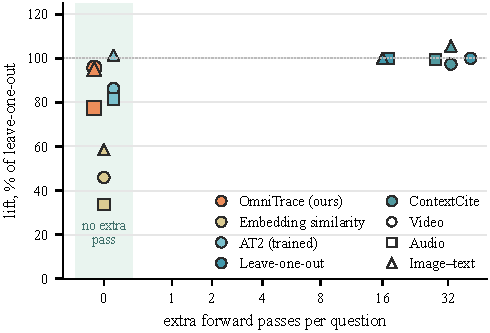
\includegraphics[width=\columnwidth]{media/figure/fig_cost.pdf}
\caption{\textbf{Faithfulness against cost} on Qwen2.5-Omni-7B (the panel of \Cref{fig:teaser}). Lift of each method as a share of leave-one-out's lift, against the extra forward passes it needs per question. Both OmniTrace variants sit in the shaded column: they read their scores from the generation pass. OmniTrace-trained needs ablation data from the same model beforehand.}
\label{fig:cost}
\end{figure}

\begin{table*}[t]
\centering
\small
\resizebox{\textwidth}{!}{% generated by analysis/paper_models.py; do not edit by hand
\begin{tabular}{llcccccc}
\toprule
\textbf{Model} & \textbf{Modality} ($n$) & Budget & Drop, top & Drop, random & Lift & Lift $>0$ & Keep gain \\
\midrule
Qwen2.5-Omni-7B & Video (246) & 10\% & 0.009 & 0.002 & 0.007 {\tiny[0.005, 0.009]} & 70\% & 0.022 {\tiny[0.006, 0.048]} \\
 &  & 20\% & 0.020 & 0.004 & 0.016 {\tiny[0.011, 0.021]} & 73\% & 0.010 {\tiny[$-$0.002, 0.021]} \\
 &  & 30\% & 0.025 & 0.009 & 0.017 {\tiny[0.013, 0.021]} & 77\% & 0.006 {\tiny[$-$0.004, 0.013]} \\
 &  & 50\% & 0.043 & 0.016 & 0.027 {\tiny[0.021, 0.034]} & 88\% & 0.005 {\tiny[$-$0.000, 0.011]} \\
 & Audio (196) & 10\% & 0.112 & 0.056 & 0.056 {\tiny[0.043, 0.069]} & 72\% & 0.042 {\tiny[0.033, 0.053]} \\
 &  & 20\% & 0.144 & 0.075 & 0.069 {\tiny[0.055, 0.086]} & 75\% & 0.066 {\tiny[0.051, 0.080]} \\
 &  & 30\% & 0.167 & 0.099 & 0.068 {\tiny[0.054, 0.083]} & 77\% & 0.073 {\tiny[0.058, 0.090]} \\
 &  & 50\% & 0.208 & 0.149 & 0.060 {\tiny[0.046, 0.073]} & 73\% & 0.080 {\tiny[0.063, 0.098]} \\
 & Image--text (400) & 1 quote & 0.314 & 0.031 & 0.282 {\tiny[0.250, 0.319]} & 92\% & 0.356 {\tiny[0.309, 0.407]} \\
 &  & 2 quotes & 0.423 & 0.076 & 0.348 {\tiny[0.310, 0.383]} & 95\% & 0.412 {\tiny[0.371, 0.456]} \\
 &  & 3 quotes & 0.485 & 0.109 & 0.377 {\tiny[0.338, 0.418]} & 94\% & 0.396 {\tiny[0.358, 0.438]} \\
\midrule
MiniCPM-o 4.5 & Video (233) & 10\% & 0.019 & 0.013 & 0.006 {\tiny[0.002, 0.010]} & 55\% & 0.010 {\tiny[$-$0.000, 0.020]} \\
 &  & 20\% & 0.046 & 0.019 & 0.027 {\tiny[0.019, 0.034]} & 73\% & 0.026 {\tiny[0.018, 0.034]} \\
 &  & 30\% & 0.078 & 0.028 & 0.050 {\tiny[0.039, 0.062]} & 79\% & 0.031 {\tiny[0.024, 0.039]} \\
 &  & 50\% & 0.123 & 0.050 & 0.073 {\tiny[0.060, 0.087]} & 85\% & 0.021 {\tiny[0.016, 0.026]} \\
 & Audio (187) & 10\% & 0.204 & 0.102 & 0.102 {\tiny[0.077, 0.131]} & 63\% & 0.060 {\tiny[0.039, 0.081]} \\
 &  & 20\% & 0.272 & 0.129 & 0.143 {\tiny[0.113, 0.174]} & 72\% & 0.106 {\tiny[0.079, 0.133]} \\
 &  & 30\% & 0.307 & 0.172 & 0.135 {\tiny[0.107, 0.162]} & 68\% & 0.128 {\tiny[0.101, 0.158]} \\
 &  & 50\% & 0.370 & 0.273 & 0.097 {\tiny[0.074, 0.121]} & 65\% & 0.125 {\tiny[0.098, 0.151]} \\
 & Image--text (400) & 1 quote & 0.145 & 0.078 & 0.067 {\tiny[0.048, 0.089]} & 58\% & 0.039 {\tiny[0.023, 0.057]} \\
 &  & 2 quotes & 0.269 & 0.164 & 0.105 {\tiny[0.076, 0.130]} & 64\% & 0.074 {\tiny[0.052, 0.096]} \\
 &  & 3 quotes & 0.414 & 0.221 & 0.194 {\tiny[0.167, 0.222]} & 75\% & 0.154 {\tiny[0.131, 0.178]} \\
\midrule
Qwen3-Omni-30B-A3B & Video (246) & 10\% & 0.022 & 0.003 & 0.019 {\tiny[0.014, 0.024]} & 70\% & 0.019 {\tiny[0.012, 0.027]} \\
 &  & 20\% & 0.038 & 0.005 & 0.033 {\tiny[0.025, 0.040]} & 74\% & 0.016 {\tiny[0.011, 0.021]} \\
 &  & 30\% & 0.047 & 0.008 & 0.038 {\tiny[0.030, 0.047]} & 76\% & 0.010 {\tiny[0.006, 0.015]} \\
 &  & 50\% & 0.061 & 0.015 & 0.046 {\tiny[0.037, 0.055]} & 77\% & 0.006 {\tiny[0.004, 0.009]} \\
 & Audio (196) & 10\% & 0.142 & 0.060 & 0.083 {\tiny[0.065, 0.103]} & 75\% & 0.059 {\tiny[0.044, 0.075]} \\
 &  & 20\% & 0.191 & 0.079 & 0.112 {\tiny[0.088, 0.137]} & 78\% & 0.097 {\tiny[0.074, 0.118]} \\
 &  & 30\% & 0.215 & 0.116 & 0.099 {\tiny[0.078, 0.125]} & 76\% & 0.100 {\tiny[0.078, 0.126]} \\
 &  & 50\% & 0.262 & 0.180 & 0.082 {\tiny[0.065, 0.100]} & 75\% & 0.094 {\tiny[0.076, 0.114]} \\
 & Image--text (400) & 1 quote & 0.276 & 0.044 & 0.232 {\tiny[0.213, 0.252]} & 96\% & 0.209 {\tiny[0.188, 0.229]} \\
 &  & 2 quotes & 0.415 & 0.099 & 0.316 {\tiny[0.294, 0.338]} & 98\% & 0.304 {\tiny[0.284, 0.329]} \\
 &  & 3 quotes & 0.495 & 0.131 & 0.363 {\tiny[0.342, 0.386]} & 99\% & 0.355 {\tiny[0.332, 0.379]} \\
\bottomrule
\end{tabular}
}
\caption{Response-level results of OmniTrace at every budget. Drops are in nats per token. Lift $>0$: share of the questions with a positive lift. Brackets: 95\% bootstrap intervals.}
\label{tab:budget}
\end{table*}

\begin{table*}[t]
\centering
\small
\setlength{\tabcolsep}{4pt}
\resizebox{\textwidth}{!}{% generated by analysis/paper_models.py; do not edit by hand
\begin{tabular}{llccccccc}
\toprule
 & & & \multicolumn{3}{c}{Lift} & \multicolumn{3}{c}{OmniTrace $-$ baseline (paired)} \\
\cmidrule(lr){4-6}\cmidrule(lr){7-9}
\textbf{Modality} & Budget & OmniTrace & Embedding & Leave-one-out & ContextCite & Embedding & Leave-one-out & ContextCite \\
\midrule
Video & 10\% & 0.007 & 0.002 & 0.014 & 0.013 & 0.005 {\tiny[0.002, 0.009]} & $-$0.007 {\tiny[$-$0.011, $-$0.005]} & $-$0.006 {\tiny[$-$0.008, $-$0.003]} \\
 & 20\% & 0.016 & 0.008 & 0.016 & 0.016 & 0.008 {\tiny[0.004, 0.013]} & $-$0.001 {\tiny[$-$0.004, 0.003]} & $-$0.000 {\tiny[$-$0.005, 0.006]} \\
 & 30\% & 0.020 & 0.012 & 0.019 & 0.022 & 0.008 {\tiny[0.004, 0.013]} & 0.001 {\tiny[$-$0.003, 0.006]} & $-$0.002 {\tiny[$-$0.006, 0.002]} \\
 & 50\% & 0.027 & 0.019 & 0.020 & 0.031 & 0.008 {\tiny[0.002, 0.014]} & 0.007 {\tiny[0.003, 0.011]} & $-$0.004 {\tiny[$-$0.009, 0.001]} \\
\midrule
Audio & 10\% & 0.060 & 0.023 & 0.090 & 0.087 & 0.037 {\tiny[0.024, 0.049]} & $-$0.030 {\tiny[$-$0.038, $-$0.023]} & $-$0.027 {\tiny[$-$0.035, $-$0.019]} \\
 & 20\% & 0.077 & 0.034 & 0.100 & 0.099 & 0.044 {\tiny[0.031, 0.057]} & $-$0.022 {\tiny[$-$0.030, $-$0.014]} & $-$0.022 {\tiny[$-$0.030, $-$0.015]} \\
 & 30\% & 0.074 & 0.037 & 0.092 & 0.096 & 0.037 {\tiny[0.025, 0.049]} & $-$0.017 {\tiny[$-$0.024, $-$0.011]} & $-$0.021 {\tiny[$-$0.028, $-$0.015]} \\
 & 50\% & 0.057 & 0.041 & 0.064 & 0.071 & 0.016 {\tiny[0.008, 0.024]} & $-$0.006 {\tiny[$-$0.011, $-$0.002]} & $-$0.014 {\tiny[$-$0.018, $-$0.009]} \\
\midrule
Image--text & 1 quote & 0.285 & 0.142 & 0.317 & 0.311 & 0.143 {\tiny[0.115, 0.172]} & $-$0.032 {\tiny[$-$0.041, $-$0.024]} & $-$0.026 {\tiny[$-$0.034, $-$0.018]} \\
 & 2 quotes & 0.351 & 0.216 & 0.368 & 0.389 & 0.135 {\tiny[0.107, 0.166]} & $-$0.018 {\tiny[$-$0.033, 0.000]} & $-$0.039 {\tiny[$-$0.054, $-$0.022]} \\
 & 3 quotes & 0.379 & 0.257 & 0.380 & 0.431 & 0.122 {\tiny[0.098, 0.148]} & $-$0.002 {\tiny[$-$0.023, 0.025]} & $-$0.052 {\tiny[$-$0.074, $-$0.033]} \\
\bottomrule
\end{tabular}
}
\caption{Lift of every method at every budget on Qwen2.5-Omni-7B, and the paired difference between OmniTrace and each baseline with its 95\% bootstrap interval. OT-trained: OmniTrace-trained (\Cref{appendix:trained}).}
\label{tab:budget_base}
\end{table*}

\Cref{tab:budget} gives the drops, lifts, and keep gains of OmniTrace at every budget, and \Cref{tab:budget_base} the comparison with the baselines.
The share of leave-one-out's lift that OmniTrace reaches grows with the budget in every modality.
On video at the 10\% budget, the keep gain against embedding similarity is dominated by one question, in which keeping the baseline's units costs 11 nats per token.

\subsection{Predicted Labels}
\label{appendix:labels}

\begin{table*}[t]
\centering
\small
\setlength{\tabcolsep}{4pt}
\resizebox{\textwidth}{!}{% generated by analysis/paper_models.py; do not edit by hand
\begin{tabular}{llcccccc}
\toprule
\textbf{Model} & \textbf{Modality} ($n$) & Units labelled & No label & Lift & Keep gain & S-lift & S-spec \\
\midrule
Qwen2.5-Omni-7B & Video (244) & 4.0 (10\%) & 2\% & 0.006 {\tiny[0.003, 0.010]} & 0.046 {\tiny[0.011, 0.112]} & 0.012 {\tiny[0.010, 0.015]} & 0.007 {\tiny[0.004, 0.009]} \\
 & Audio (196) & 2.6 (16\%) & 14\% & 0.079 {\tiny[0.061, 0.098]} & 0.077 {\tiny[0.061, 0.096]} & 0.125 {\tiny[0.109, 0.145]} & 0.106 {\tiny[0.082, 0.133]} \\
 & Image--text (400) & 3.1 (21\%) & 0\% & 0.364 {\tiny[0.326, 0.400]} & 0.393 {\tiny[0.352, 0.439]} & 0.411 {\tiny[0.389, 0.433]} & 0.240 {\tiny[0.213, 0.269]} \\
\midrule
MiniCPM-o 4.5 & Video (233) & 5.2 (13\%) & 0\% & 0.006 {\tiny[0.002, 0.010]} & 0.006 {\tiny[$-$0.004, 0.016]} & 0.014 {\tiny[0.008, 0.020]} & 0.008 {\tiny[0.002, 0.015]} \\
 & Audio (187) & 1.6 (15\%) & 0\% & 0.073 {\tiny[0.047, 0.101]} & 0.042 {\tiny[0.022, 0.065]} & 0.080 {\tiny[0.059, 0.100]} & 0.047 {\tiny[0.011, 0.088]} \\
 & Image--text (400) & 3.1 (21\%) & 0\% & 0.170 {\tiny[0.142, 0.199]} & 0.149 {\tiny[0.124, 0.174]} & 0.458 {\tiny[0.436, 0.479]} & 0.344 {\tiny[0.319, 0.367]} \\
\midrule
\bottomrule
\end{tabular}
}
\caption{Causal test of the labels of \Cref{eq:label} at $\tau=1.5$. Units labelled: mean number per response and share of the candidate units. No label: responses whose response-level label is empty. Lift and keep gain compare the labelled units with random units of the same count.}
\label{tab:labels}
\end{table*}

\Cref{tab:labels} tests the labelled sets.
All lifts, sentence lifts, and sentence specificities are above zero.
The keep gain on video is positive but not reliable for MiniCPM-o~4.5, and for Qwen2.5-Omni its mean is raised by one question.

\subsection{Label Threshold}
\label{appendix:threshold}

For image--text input, $\tau=1.5$ gives the highest mean F1 against the gold quotes on 200 development questions that are disjoint from the test questions.
Audio and video have no usable labels for this, so we compared thresholds by the causal effect of the labelled sets on a random fifth of the questions (54 video, 53 audio), which is excluded from all results.
No threshold was reliably better than 1.5 there; lower values scored slightly higher, so this check supports 1.5 as a safe choice and does not show that it is optimal.
MiniCPM-o~4.5 uses the same value without any check.

\subsection{Variants and Human-Evidence Units}
\label{appendix:variants}

\begin{table*}[t]
\centering
\small
\setlength{\tabcolsep}{4.2pt}
\resizebox{\textwidth}{!}{% generated by analysis/paper_models.py; do not edit by hand
\begin{tabular}{lcccccccccccc}
\toprule
 & \multicolumn{4}{c}{\textbf{Video}} & \multicolumn{4}{c}{\textbf{Audio}} & \multicolumn{4}{c}{\textbf{Image--text}} \\
\cmidrule(lr){2-5}\cmidrule(lr){6-9}\cmidrule(lr){10-13}
 & Lift & Keep & S-lift & S-spec & Lift & Keep & S-lift & S-spec & Lift & Keep & S-lift & S-spec \\
\midrule
\multicolumn{13}{>{\columncolor{gray!15}}l}{\textit{Qwen2.5-Omni-7B} \;($n$ = 246, 196, 400)}\\
\textbf{OmniTrace} & 0.016 & 0.010 & 0.015 & 0.007 & 0.069 & 0.066 & 0.103 & 0.084 & 0.348 & 0.412 & 0.375 & 0.245 \\
\;argmax tracing + curation & 0.009\mdn & 0.008 & 0.010\mdn & 0.004\mdn & 0.067 & 0.064 & 0.096\mdn & 0.081 & 0.346 & 0.420 & -- & -- \\
\;last layer only & 0.014 & 0.010 & -- & -- & 0.048\mdn & 0.046\mdn & -- & -- & 0.306\mdn & 0.380\mdn & -- & -- \\
\;per-token mean & -- & -- & -- & -- & -- & -- & -- & -- & 0.224\mdn & 0.255\mdn & 0.286\mdn & 0.214\mdn \\
Human-evidence units & 0.009\mdn & -- & -- & -- & -- & -- & -- & -- & 0.211\mdn & -- & -- & -- \\
\midrule
\multicolumn{13}{>{\columncolor{gray!15}}l}{\textit{MiniCPM-o 4.5} \;($n$ = 233, 187, 400)}\\
\textbf{OmniTrace} & 0.027 & 0.026 & 0.029 & 0.013 & 0.143 & 0.106 & 0.120 & 0.055 & 0.105 & 0.074 & 0.158 & 0.098 \\
\;argmax tracing + curation & 0.027 & $-$0.051\mdn & 0.025 & $-$0.001\mdn & 0.020\mdn & 0.001\mdn & 0.021\mdn & 0.006\mdn & 0.079\mdn & 0.058\mdn & -- & -- \\
\;last layer only & 0.025 & 0.005\mdn & -- & -- & 0.091\mdn & 0.055\mdn & -- & -- & 0.092 & 0.056 & -- & -- \\
\;per-token mean & -- & -- & -- & -- & -- & -- & -- & -- & 0.083 & 0.057 & 0.188\mup & 0.165\mup \\
Human-evidence units & 0.043\mup & -- & -- & -- & -- & -- & -- & -- & 0.334\mup & -- & -- & -- \\
\midrule
\multicolumn{13}{>{\columncolor{gray!15}}l}{\textit{Qwen3-Omni-30B-A3B} \;($n$ = 196, 400)}\\
\textbf{OmniTrace} & -- & -- & -- & -- & 0.112 & 0.097 & 0.095 & 0.065 & 0.316 & 0.304 & 0.448 & 0.309 \\
\;argmax tracing + curation & -- & -- & -- & -- & 0.112 & 0.105\mup & 0.087\mdn & 0.068 & 0.323 & 0.322\mup & -- & -- \\
\;last layer only & -- & -- & -- & -- & 0.045\mdn & 0.030\mdn & -- & -- & 0.125\mdn & 0.124\mdn & -- & -- \\
\;per-token mean & -- & -- & -- & -- & -- & -- & -- & -- & 0.240\mdn & 0.233\mdn & 0.381\mdn & 0.297\mdn \\
Human-evidence units & -- & -- & -- & -- & -- & -- & -- & -- & 0.267\mdn & -- & -- & -- \\
\bottomrule
\end{tabular}
}
\caption{OmniTrace on three models, variants that change one design choice, and human-marked evidence.
Lift and Keep: lift and keep gain at response level (20\% of the duration; 2 quotes); S-lift and S-spec: sentence lift and specificity, in nats per token.
\mdn / \mup: reliably lower / higher than OmniTrace on the same questions or sentences.
\emph{Argmax tracing + curation} traces each token to its highest-attention position and filters the votes; \emph{last layer only} and \emph{per-token mean} change one choice in \Cref{eq:mass}.
\emph{Human-evidence units} hides the units annotators marked (not available for audio); their number differs from the budget, so their lift is against random sets of their own size.}
\label{tab:models}
\end{table*}

\begin{figure}[t]
\centering
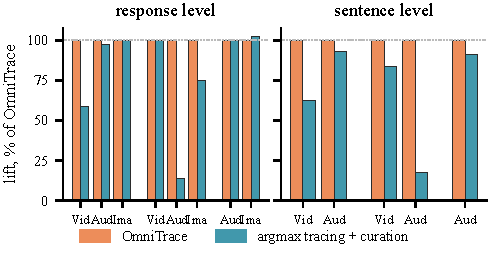
\includegraphics[width=\columnwidth]{media/figure/fig_transfer.pdf}
\caption{Lift of argmax tracing with curation as a share of OmniTrace's lift. In each panel the groups of bars are, from left to right, Qwen2.5-Omni-7B, on which the variant was developed, MiniCPM-o~4.5, and Qwen3-Omni-30B.}
\label{fig:transfer}
\end{figure}

\Cref{tab:models} compares OmniTrace with variants that change one design choice, and \Cref{fig:transfer} shows the comparison with hard tracing.
On Qwen2.5-Omni, argmax tracing with curation is level with OmniTrace on audio and image--text input and behind on video.
On MiniCPM-o~4.5 it loses most of its effect on audio, is behind on image--text input, and on video its top units are worse to keep than random ones.
On Qwen3-Omni-30B it is level with OmniTrace in lift on audio and image--text input, slightly ahead in keep gain, and behind at sentence level on audio; on video it keeps 60\% of the lift, as on Qwen2.5-Omni.
Using the last layer alone is reliably worse on audio for all three models, and on Qwen3-Omni it loses more than half of the lift in every modality.

The last rows hide the units that annotators marked.
On Qwen2.5-Omni, the units OmniTrace selects have a larger lift than the human-marked ones.
On Qwen3-Omni-30B the same holds for image--text input (0.316 against 0.267), and on video the two are close (0.033 against 0.027).
On MiniCPM-o~4.5 the order is reversed, most clearly on image--text input: there OmniTrace finds units that matter, but not the ones that matter most.

\subsection{Unit Size}
\label{appendix:size}

\begin{table}[t]
\centering
\tablesize
\setlength{\tabcolsep}{3.5pt}
% source: analysis/out/qwen2.5-omni-7b/unit_size.md (A)
\begin{tabular}{lccc}
\toprule
\textbf{Ranking} & $\rho$(score, size) & Top-1 size & Image share\\
\midrule
OmniTrace (sum) & $+$0.51 & 1.94 & 0.59\\
Per-token mean & $-$0.60 & 0.44 & 0.11\\
Leave-one-out & $+$0.09 & 1.62 & 0.48\\
ContextCite & $+$0.14 & 1.65 & 0.52\\
OmniTrace-trained & $+$0.08 & 1.71 & 0.52\\
Human evidence & $+$0.25 & 1.85 & 0.67\\
\bottomrule
\end{tabular}
\caption{Unit size on image--text input (Qwen2.5-Omni-7B). $\rho$: rank correlation between a quote's score and its token count, per question. Top-1 size: tokens of the top quote over the mean quote size. Image share: share of images among the top-ranked quotes.}
\label{tab:size}
\end{table}

\Cref{tab:size} gives the numbers behind \Cref{sec:size}. The per-token mean ranks short passages first and rarely an image. On MiniCPM-o~4.5 the mean is better than the sum at sentence level (\Cref{tab:models}), so the best correction for size depends on the model.

\subsection{Unit Granularity}
\label{appendix:granularity}

The score of a merged unit is the sum of its parts, but a selected set can still change with the unit length.
We merge one-second units into two- and four-second units and select the top 20\% of the duration again.
On video the selected time overlaps the one-second selection with IoU 0.60 and 0.50, where random rankings give 0.15; on audio the values are 0.53 and 0.42.
The selection is far from arbitrary but not invariant, so the unit length should be fixed and reported.

\subsection{Attribution Strength}
\label{appendix:flagging}

At sentence level, the attention mass a sentence places on the sources correlates with how much the sentence depends on them (rank correlation 0.60 on audio and image--text input, 0.26 on video, Qwen2.5-Omni).
At response level, a low share of mass on the audio flags wrong answers on Qwen2.5-Omni (AUROC 0.74), but not in the other modalities and not on MiniCPM-o~4.5.
Attribution strength thus indicates whether a sentence draws on the sources; it is not a general detector of wrong answers.

\section{Answer Accuracy of Long Answers}
\label{appendix:judge}

MMDocRAG answers are free text, so we grade them with an LLM judge (\texttt{claude-opus-5-5}).
The judge sees the question, the short and long reference answers, and the model's response, and returns \emph{correct} (all facts the reference needs), \emph{partial} (some facts right, at least one missing or wrong), or \emph{incorrect}. It does not see the quotes or images.
For Qwen2.5-Omni-7B, 374 of the 400 responses received a verdict: 23.8\% correct, 43.0\% partial, 33.2\% incorrect.
For MiniCPM-o~4.5 (400 verdicts): 50.5\% correct and 35.3\% partial.
For Qwen3-Omni-30B (400 verdicts): 54.0\% correct and 32.8\% partial.
The accuracy is used only to describe the models and to select correctly answered questions in \Cref{sec:agreement}.

\section{Data and Code}
We will release the code of OmniTrace, the causal tests, and the baselines, together with the question lists and the model responses used in this paper. The datasets keep the licenses of their creators.

\end{document}
